\begin{frame}[t,fragile]{Ausgangspunkt}
\begin{itemize}
\item Betriebswirtschaftliche Software
\item Extrem schlechte Codequalität (sowohl messbar als auch erfahrbar)
\item Funktionalität eines Moduls musste verändert werden
\begin{itemize}
\item Bugfixing
\item neue Features
\item bessere Tests
\end{itemize}
\end{itemize}

$\Rightarrow$ Wir mussten einen Umbau vornehmen
\end{frame}

\begin{frame}[t,fragile]{Vorhandene Codestruktur}
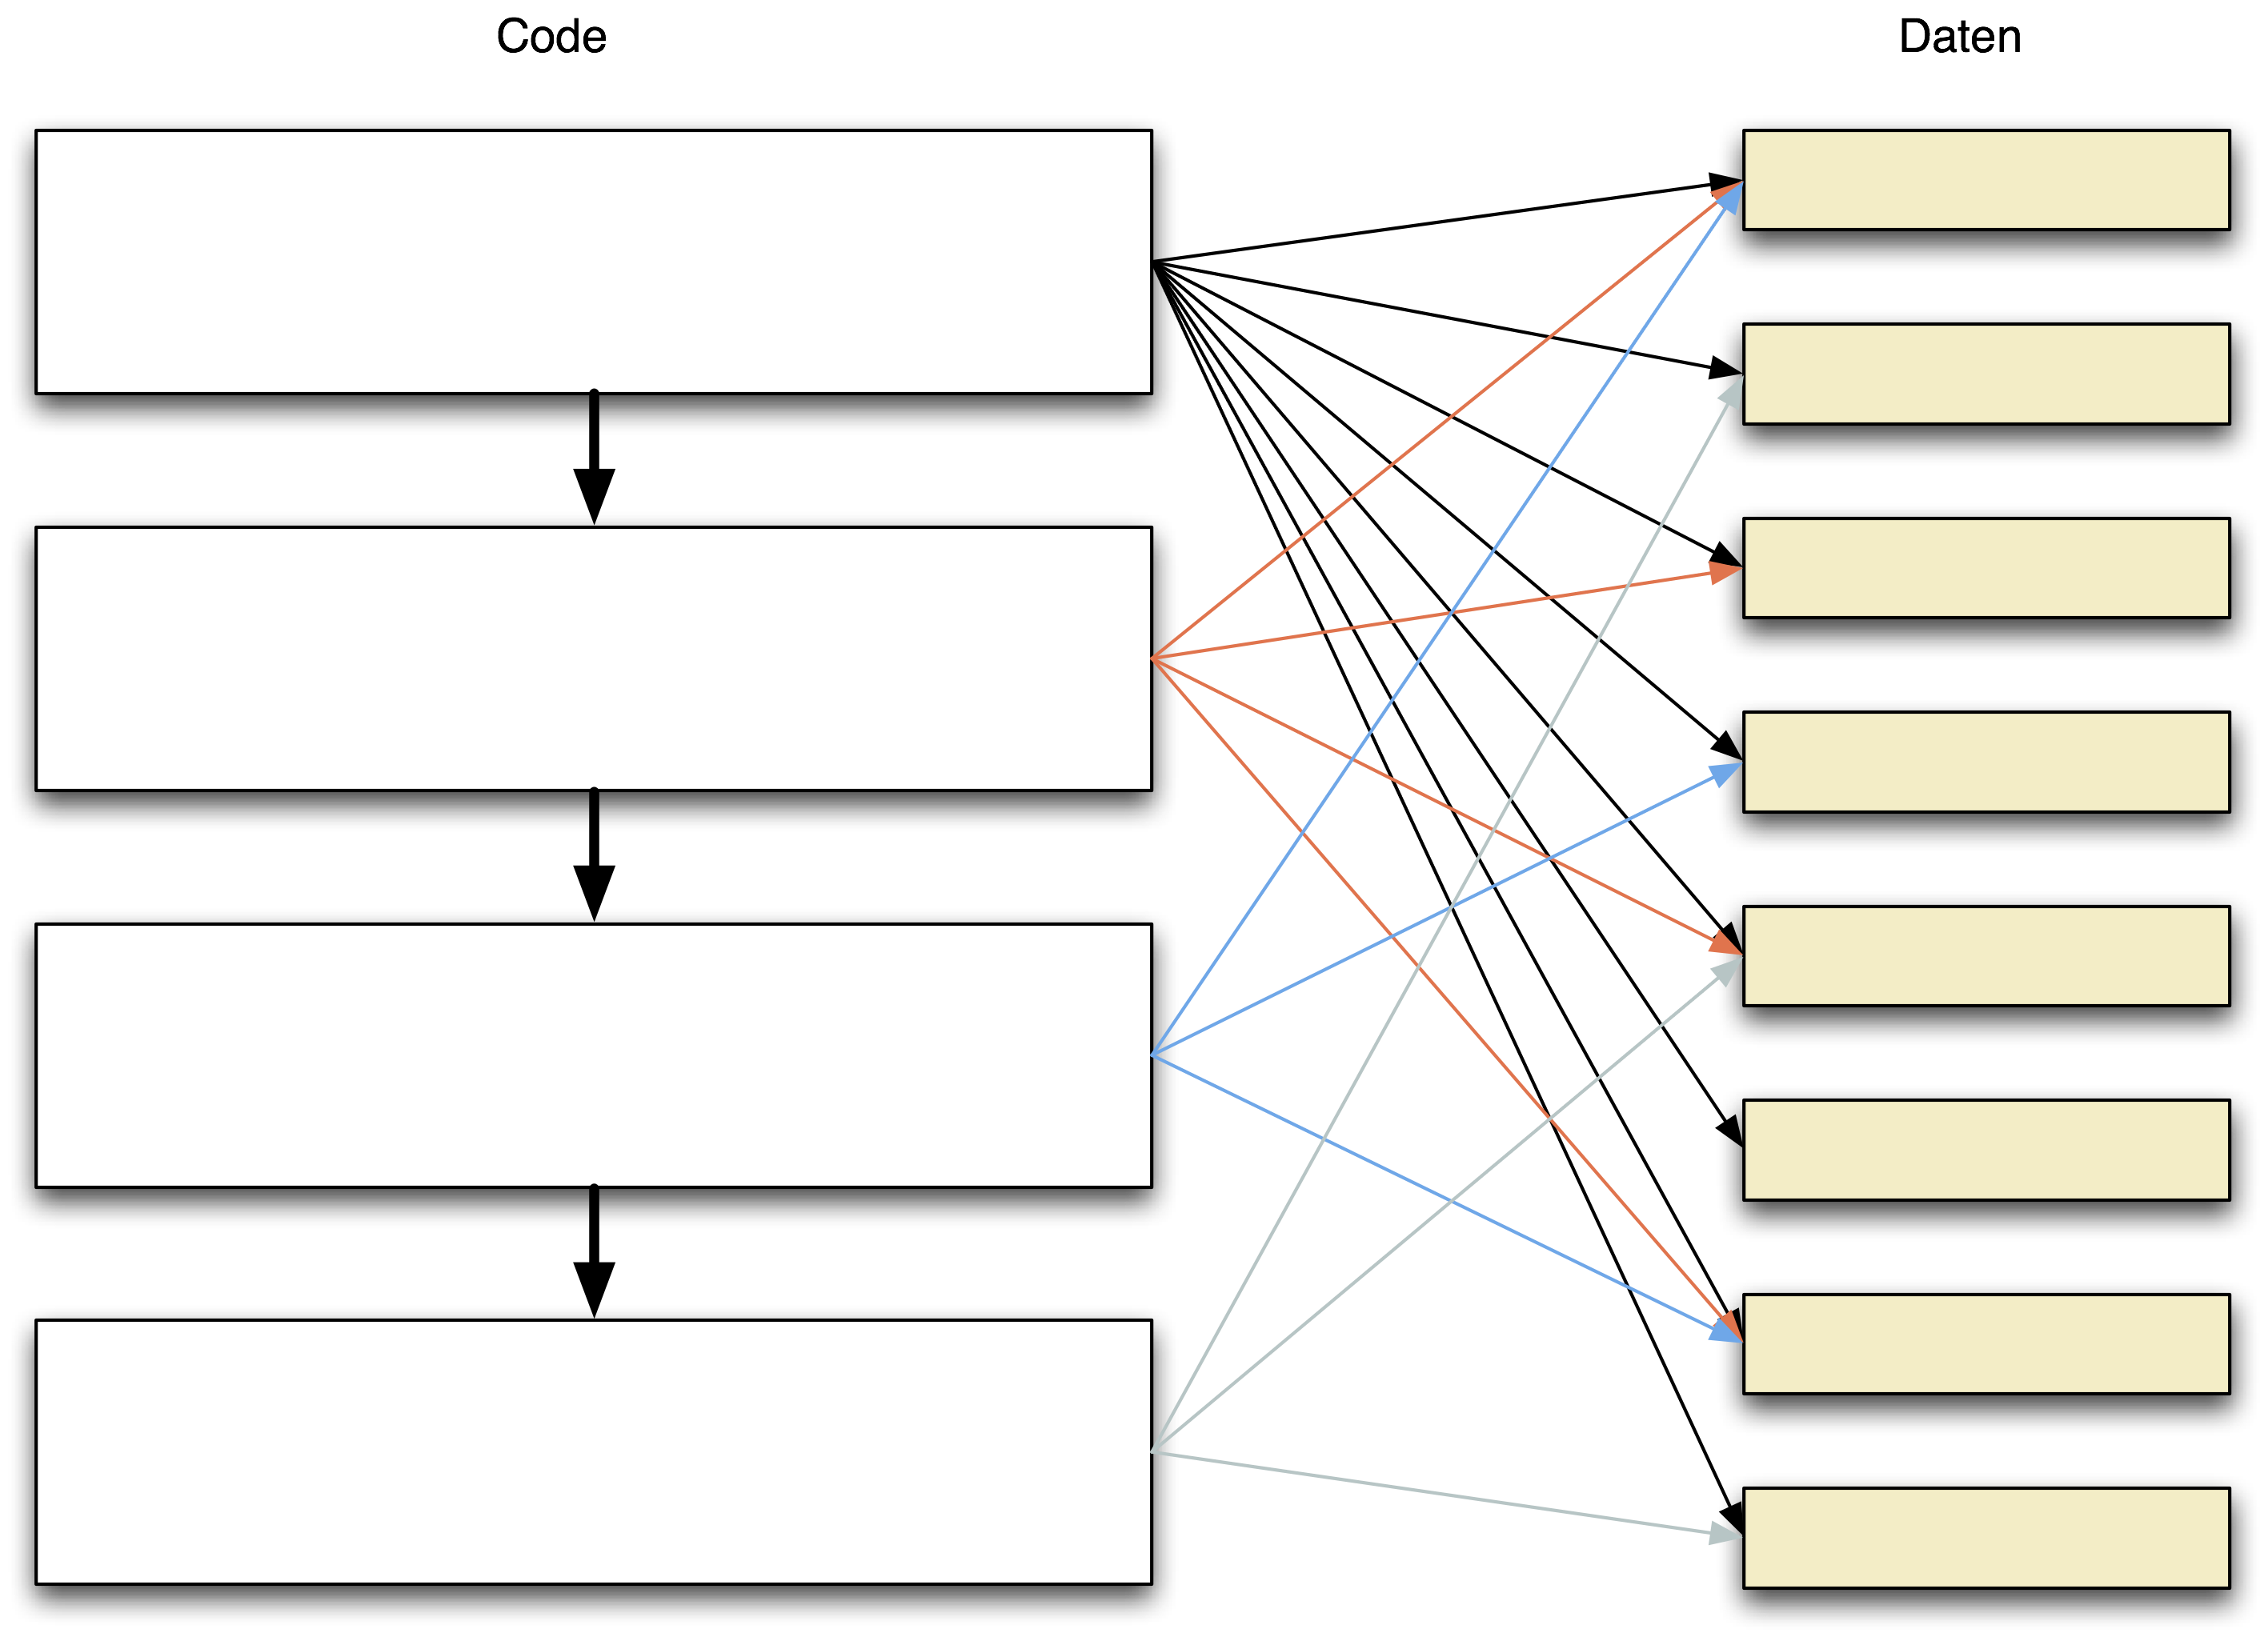
\includegraphics[width=.8 \paperwidth]{Codestruktur.png}
\end{frame}

\begin{frame}[t,fragile]{Probleme der vorhandenen Codestruktur}
\begin{itemize}
\item Code schreibt Werte in separate Datenobjekte (\glqq Push\grqq{})
\item Mehrfache Schreibzugriffe auf denselben Wert
\item Codeteile greifen auf vorher geschriebene Werte zu
\item Code ist getrieben vom Blick von innen: Was muss ich alles in Summe tun, um eine Menge von Ergebnissen abliefern zu können?
\end{itemize}
\end{frame}


\begin{frame}[t,fragile]{Vorgehensweise}
\begin{itemize}
\item Beibehalten der externen API
\item Feature-Toggle zum Vergleichen der alten und der neuen Version
\item Umbau:
\begin{itemize}
\item Rein strukturell
\item Fachlich motiviert
\end{itemize}

\item Ziel:
\begin{itemize}
\item On-Demand-Ermittlung aller Werte (\glqq Pull\grqq{})
\item Werte-Caching mittels Lazy-Pattern
\end{itemize}
\end{itemize}
\end{frame}

\begin{frame}[t,fragile]{Unser Ansatz}
\begin{itemize}
\item Unser größter Fehler: Aufbau der Zielstruktur und Neuimplementierung der Logik anhand einer vom Code unabhängigen Spezifikation
\end{itemize}
$\Rightarrow$ Viele Abweichungen in den Ergebnissen, lange Phase der fachlichen Klärung
\end{frame}

%\begin{frame}[t,fragile]{}
%\begin{itemize}
%\item
%\end{itemize}
%\end{frame}
%
%\begin{frame}[t,fragile]{}
%\begin{itemize}
%\item
%\end{itemize}
%\end{frame}
%
%\begin{frame}[t,fragile]{}
%\begin{itemize}
%\item
%\end{itemize}
%\end{frame}
%
%\begin{frame}[t,fragile]{}
%\begin{itemize}
%\item
%\end{itemize}
%\end{frame}

\begin{frame}[t,fragile]{Ein besserer / ... Ansatz}
\begin{itemize}
\item Codeveränderungen betreffen lediglich die Struktur, NICHT die Logik
\item Wenn gleichzeitig Umbauten der Logik erforderlich sind:
\begin{itemize}
\item Vorsichtig herangehen
\item Kleine Schritte gehen
\item Veränderungen der Logik entweder komplett vorher oder nachher durchführen, NICHT während des strukturellen Umbaus
\end{itemize}

\item Vorhandene Regressionstests auf Vollständigkeit prüfen (Code Coverage untersuchen)
\item Bei geringer Coverage Regressionstests ergänzen oder komplett neu erstellen
\end{itemize}
\end{frame}



\begin{frame}[t,fragile]{Wozu das Ganze?}
\begin{itemize}
\item Umbau der Struktur: damit die vorhandene Implementierung der Sachlichkeit besser sichtbar wird und isoliert vorliegt
$\Rightarrow$ ermöglicht später gezielte Änderung einzelner Aspekte der Fachlichkeit
\item Trennung der Aspekte: damit die Regressionstests bei den Strukturveränderungen gültig bleiben und alle Veränderungen im Verhalten anzeigen
\item Fachlich motiviert, Blick von außen aus Sicht der Ergebnisse:
\begin{itemize}
\item Welche Werte will ich haben?
\item Wie berechnet sich welcher Wert?
\item Welche Arten von Ergebniswerten gibt es? Gemeinsamkeiten, Unterschiede?
\end{itemize}
\end{itemize}
\end{frame}

\begin{frame}[t,fragile]{Umbau: Vorbereitung}
\begin{itemize}
\item Existierenden Code duplizieren
\item Feature Toggle an den Aufrufstellen einbauen
\end{itemize}
\end{frame}
 
\begin{frame}[t,fragile]{Vorarbeiten}
\begin{itemize}
\item Java-Datumsarithmetik kapseln, z.~B.
\begin{itemize}
\item Joda Time
\item Eigene Klassen
\end{itemize}
\item Namensgebung von Variablen verbessern
\end{itemize}
\end{frame}

\begin{frame}[t,fragile]{Strukturellen Code isolieren}
\begin{itemize}
\item Inline method: Nur noch eine Methode
\item Schleifen über Ergebnisstruktur nach außen bringen
\item Schleifen vereinheitlichen
\end{itemize}
\end{frame}

\begin{frame}[t,fragile]{Aspekte isolieren}
\begin{itemize}
\item Schleifenrumpf in eigene Klasse mit einer Methode extrahieren
\item Pro Ergebniswert ein Duplikat dieser Methode
\item Jeweils Irrelevantes aus den Methoden entfernen
\end{itemize}
\end{frame}

\begin{frame}[t,fragile]{Zielstruktur aufbauen}
\begin{itemize}
\item Zuerst nur als Gerüst mit Befüllung von außen
\item Berechnung \textbf{eines} Werts in die Zielstruktur übertragen
\item Prüfen der Tragfähigkeit der Zielstruktur
\end{itemize}
\end{frame}

\begin{frame}[t,fragile]{Vervollständigung}
\begin{itemize}
\item Wert für Wert in die Zielstruktur übertragen
\item Parallel dazu Unit-Tests aufbauen
\item Refactoring: 
\begin{itemize}
\item Extrahieren von Methoden
\item Zusammenfassen gleicher Funktionalität
\item Generelle Aufräumarbeiten
\end{itemize}
\item Klärung fachlicher Unklarheiten, Korrektur der Logik
\end{itemize}
\end{frame}

%\begin{frame}[t,fragile]{}
%\begin{itemize}
%\item
%\end{itemize}
%\end{frame}
%
%\begin{frame}[t,fragile]{}
%\begin{itemize}
%\item
%\end{itemize}
%\end{frame}
%
%\begin{frame}[t,fragile]{}
%\begin{itemize}
%\item
%\end{itemize}
%\end{frame}
%
%\begin{frame}[t,fragile]{}
%\begin{itemize}
%\item
%\end{itemize}
%\end{frame}
%
%\begin{frame}[t,fragile]{}
%\begin{itemize}
%\item
%\end{itemize}
%\end{frame}

